\chapter{Related Work}
\label{Chapter:RelatedWork}

To understand how software project telemetry relates to other research, it is useful to think in terms of two concepts: \textit{measurement machinery} and \textit{process methodology}. Measurement machinery refers to how software metrics are collected and analyzed. In software project telemetry, sensors collect metrics automatically and unobtrusively. Metrics are abstracted into telemetry streams, charts, and reports, representing high-level perspectives on software development. Project management and process improvement decisions are based on trends detected in telemetry streams. Process methodology refers to specific techniques used to improve the quality of software development effort. Software project telemetry employs cycles of process problem detection, improvement hypothesis generation, change implementation, and hypothesis validation to empirically guide project management and process improvement decision-making.

This chapter compares and contrasts software project telemetry to other approaches to measurement machinery and process methodology. Some approaches, such as the Personal Software Process (PSP) \cite{Humphrey:1995, Humphrey:1996}, can be compared to software project telemetry with respect to both measurement machinery and process methodology. Other approaches, such as the Constructive Cost Model (COCOMO)  \cite{Cocomo:1981, Cocomo:2000}, are only comparable with respect to measurement machinery. Still others, such as the Goal-Quality-Metric paradigm (GQM) \cite{Basili:1988, Basili:1992}, and the Software Capability Maturity Model (CMM) \cite{Paulk:1993, SEI:1995}, are only comparable with respect to process methodology. 


This chapter proceeds with an overview of software measurement theory in Section \ref{RelatedWork:MeasurementOverview}, which serve as the foundation of any software measurement programs.
Section \ref{RelatedWork:PSP} discusses the Personal Software Process. 
Section \ref{RelatedWork:COCOMO} discusses process prediction models, especially the Constructive Cost Model. 
Section \ref{RelatedWork:GQM} discusses the Goal-Question-Metric paradigm.
Section \ref{RelatedWork:CMM} discusses maturity frameworks, especially the Software Capability Maturity Model.
Section \ref{RelatedWork:Summary} concludes the chapter with a summary.


%This chapter gives a brief review of related work. It is organized as follows. 
%Section \ref{RelatedWork:MeasurementOverview} gives an overview of software measurement. 
%Section \ref{RelatedWork:GQM} introduces the Goal-Question-Metric paradigm, which offers a goal-driven approach to determine the needed metrics in a measurement program.
%Section \ref{RelatedWork:DataCollection} describes and compares different software metrics collection techniques. 
%The rest of the sections are on researches related to metrics data analysis.  The term ``metrics analysis'' is used broadly in this chapter, it includes all researches that uses software metrics data.
%Section \ref{RelatedWork:ProcessReasearch} discusses researches on software process modeling. 
%Section \ref{RelatedWork:ProcessImprovement} discusses software process improvement and assessment frameworks.
%Section \ref{RelatedWork:PredictionModel} discusses software prediction models.
%Section \ref{RelatedWork:Summary} concludes the chapter with a summary.

 
%This chapter gives a brief overview of literature with respect to software metrics and process improvement programs. Three perspectives on software process improvement programs are identified: goal-based improvement, standard-based improvement and model-based improvement.
%
%All software process improvement programs rely on software metrics, which measures software products as well as the processes by which they are developed. There are a broad range of software metrics to choose from depending on what software attributes we want to quantify. Generally they can be organized into two categories \cite{Fenton:1997}. 
%\begin{itemize}
%  \item Internal software product metrics such as size, complexity and modularity.
%  \item External software process metrics such as effort, productivity, quality and reliability.
%\end{itemize}


%%Reference: A general overview of software measurement.
%%N. E. Fenton and S. L. Pfleeger 1997
%%Software Metrics: A Rigorous and Practical Approach,
%%second edition, Thomson Computer Press 

%%Reference: In-depth discussion of the history and theory of software measurement.
%%H. Zuse
%%A Framework of Software Measurement, 
%%Walter de Gruyter

%%Reference: An overview of software process improvement approaches.
%%H. E. Thomson and P. Mayhew 1997
%%Approaches to Software Process Improvement
%%Software Process - Improvement and Practice

%%Reference: An extensive overview of maturity-based process improvement methodologies.
%%S. Zahran 1997
%%Software Process Improvement: Practical Guidelines for Business Success
%%Addison Wesley






%%%%%%%%%%%%%%%%%%%%%%%%%%%%%%%%%%%%%%%%%%%%%%%%%%%%%%%%%%%%%%%%%%%%%%%%%%%%%%
%
%  General software measurement theory:
%       1. Entity (Product/Process);  Attribute (Internal/External)
%       2. Representation theory; Measurement Scale
%       3. Metrics Validation (Meausrement system / Prediction system) (taken out)
%
%%%%%%%%%%%%%%%%%%%%%%%%%%%%%%%%%%%%%%%%%%%%%%%%%%%%%%%%%%%%%%%%%%%%%%%%%%%%%%

%\begin{quote}
%  \textit{When you can measure what you are speaking about, and express it into numbers, you know something about it; but when you cannot measure it, when you cannot express it in numbers, your knowledge is of a meager and unsatisfactory kind: It may be the beginning of knowledge, but you have scarcely in your thoughts advanced to the stage of science.}
%\begin{flushright}\textit{--- Lord Kevin, 1891 \cite{Kelvin:1891}}\end{flushright}
%\end{quote}


\section{Software Measurement Theory}  \label{RelatedWork:MeasurementOverview}

As noted by DeMarco \cite{DeMarco:1982}, \textit{You can neither predict nor control what you cannot measure}. Measurement is the first step of transforming software engineering from an art where the success of a project depends on competence and commitment of individual developers, to a scientific discipline where project outcome is both predictable and controllable.

Measurement is ``the process by which numbers or symbols are assigned to attributes of entities in the real world in such a way as to describe them according to clearly defined rules'' \cite{Fenton:1997}. This definition depends on two related concepts: \textit{entity} and \textit{attribute}. 
An entity can be a physical object such as a program, an event such as a release milestone, and an action such as testing software. In software measurement, entities are usually divided into 2 categories: \textit{software product} and \textit{software process}. 
An attribute is a property of the entity, such as the size a program, the size of the test scripts, and the time required to finish a milestone. Attributes are generally divided into 2 categories: \textit{internal attributes} and \textit{external attributes}. Measures for internal attribute can be computed based on the entity itself; while measures for external attribute depends on both the entity and the environment in which the entity resides. 
The resulting classification scheme is depicted in Table \ref{table:Software-Measurement-Classification}.

\begin{table}[tbp]
	\centering
		\begin{tabular}{|p{0.30\textwidth}|p{0.30\textwidth}|p{0.30\textwidth}|} 
			\hline
			{} & \textbf{Internal Attributes} & \textbf{External Attributes} \\
			\hline
			\textbf{Software Product} & size, complexity, cohesion, coupling, etc. & quality, reliability, maintainability, portability, etc. %\cite{Musa:1987}
			\\
			\hline
			\textbf{Software Process} & {} & time, effort, cost, etc. \\
			\hline
		\end{tabular}
	\caption{Software Measurement Classifications}
	\label{table:Software-Measurement-Classification}
\end{table}

%Software project telemetry embraces measurement at the core of its operation: sensors collect metrics, reducers abstract metrics into telemetry streams, and telemetry language allows user to compose telemetry charts and reports from telemetry streams.




%\subsection{The Representational Theory and Measurement Scales}

The representation theory formalizes the process of mapping from an empirical relation system to a numerical relation system. Under this theory, a ``measure'' is nothing but the number assigned to describe some attribute of an entity by the mapping process. However, the theory does imply that not all mappings are the same. For example, the result of a sports competition, the first place, the second place, and the third place are usually mapped to real number \textit{1}, \textit{2}, and \textit{3} respectively. Since sports competition result contains only ordinal information, it is equally valid to use \textit{1}, \textit{10}, and \textit{100} as the mapping result. It is meaningless to add these numbers. This simple example shows that not all valid mathematical analyses in numerical relation system are valid in the original empirical relation system.

Formally, the measurement mapping together with the associated empirical and numerical relation systems is referred to as the ``measurement scale''. It is the measurement scale that determines valid mathematical operations that can be performed. In general, people classify measurement scale into 4 types with increasing level of restrictiveness: \textit{nominal}, \textit{ordinal}, \textit{interval}, and \textit{ratio}.

\begin{itemize}
	\item \textit{Nominal Scale} --- The empirical relation system consists only of different classes. An example is the type of software fault, such as \textit{specification}, \textit{design}, and \textit{coding}. There is no notion of ordering between different classes. As a result, any distinct numbering representation is a valid measure.
	
	\item \textit{Ordinal Scale} --- It preserves ordering. The empirical relation system consists of classes that are ordered. An example is defect severity, such as \textit{minor}, \textit{major}, and \textit{critical}. Any mapping that preserves the ordering is a valid mapping, and the numbers represent ranking only. Arithmetic operations, such as \textit{addition}, \textit{subtraction}, \textit{multiplication}, and \textit{division}, have no meaning.
	
	\item \textit{Interval Scale} --- It preserves not only ordering but also differences. The difference between any two of the ordered classes in the range of the mapping is the same. Only \textit{addition} and \textit{subtraction} are valid. For example, when talking about time, we can say that ``year 2000 is 1000 years later than year 1000'', and ``year 3000 is 1000 years later than year 2000'', but we cannot say that ``year 2000 is twice as late as year 1000''. 
	
	\item \textit{Ratio Scale} --- It preserves ordering, differences, and ratios. The measurement starts from a zero element representing total lack of attribute, and increases at equal intervals know as units. All arithmetic operations, \textit{addition}, \textit{subtraction}, \textit{multiplication}, and \textit{division}, can be meaningfully applied. Using the length of software code as an example, we can say that ``this code contains no lines'', ``this code contains 20 more lines than that code'', and ``this code contains twice as many lines as that code''. 

\end{itemize}


 

In the current implementation of software project telemetry, mathematical manipulation of software metrics occurs at two consecutive stages: \textit{reduction processing} and \textit{telemetry language processing}. 

Reduction processing is the process of generating basic telemetry streams by filtering, synthesizing, and aggregating raw metrics collected by sensors. Reduction functions implement different reduction behaviors. They form the lowest level, atomic ``build blocks'' of the software project telemetry infrastructure observable by an end user. Though data points in telemetry streams are mapped to real numbers by reduction functions, they can be of any measurement scale in theory. The reduction process itself is treated as a black box by the infrastructure, and it is the responsibility of individual reduction function implementation to ensure that sensor data are manipulated in a meaningful way. 

Telemetry language processing acts on telemetry streams. The data points in telemetry streams are treated as if there were of ratio scale by the language interpreter. As a result, the language allows addition, subtraction, multiplication, and division between telemetry streams. %In current reference implementation, the interpreter does not perform semantic check. As a result, a user can apply meaningless operations. For example, it is possible to add two telemetry streams, one representation system test coverage, the other representing system size. This is the limitation on the language processing implementation, instead of the limitation on software project telemetry.

Theoretically, there is possibility of scale type mismatch between reduction processing and telemetry language processing. Telemetry language processing assumes that all data points in telemetry streams are of ratio scale, which cannot be guaranteed by reduction processing. This could possibly lead to problems, because telemetry language might allow meaningless mathematical operations to be applied. The problem could be solved by introducing measurement scale type system into the telemetry language, requiring all reduction functions to tag telemetry streams with scale types, and doing additional check during language interpretation. However, doing so complicates the language design and its implementation. Currently, software project telemetry takes a more pragmatic approach by relying on end users to use telemetry language in a meaningful way. In the future, the usage pattern of the language needs to be studied in order to determine the cost and benefit of introducing scale type system into the language.

%However, doing so would unnecessarily complicate software project telemetry system while achieving little benefit. In reality, scale type mismatch seldom occurs, because most software metrics are of ratio scale. Even if it does occur, most telemetry streams that do not make sense can be spotted right away. As a result, 






%%%%%%%%%%%%%%%%%%%%%%%%%%%%%%%****************************************
%
% Seems to be irrelevant stuff, the entire subsection is commented out.
%
%%%%%%%%%%%%%%%%%%%%%%%%%%%%%%%%%%%%%%%%%%%%%%%%%%%%%%%%%%%%%%%%%%%%%%%%

%%%%%%%%%%%%%%%%%%%%%%%%%%%%%%%%%%%%%%%%%%%%%%%%%%%%%%%%%%%%%%%%%%%%%%%%%%%%%%
%               S T A R T   O F   C O M M E N T
%%%%%%%%%%%%%%%%%%%%%%%%%%%%%%%%%%%%%%%%%%%%%%%%%%%%%%%%%%%%%%%%%%%%%%%%%%%%%%
\begin{comment}
\subsection{Metrics Validation}  \label{RelatedWork:MetricsExternalValidation}

Software metrics need to be validated before they can be used. Since telemetry streams are constructed from metrics, software project telemetry is closely related to metrics validation. There are 3 types of validation people are most concerned about: \textit{measurement}, \textit{internal}, and \textit{external}. As a side note, it appears that the definitions of different types of validity are not consistent in existing literature. This dissertation sticks to the following definitions:

\begin{itemize}
	\item \textit{Measurement Validity} --- It refers to whether we are measuring what we are supposed to measure and how accurate the measurement is.
	\item \textit{Internal Validity} --- It is related to causality, in other words, whether certain treatment or attribute causes the observed outcome.
	\item \textit{External Validity} --- It refers to the extent to which the results generated in one setting can be expected to hold true in other settings.
\end{itemize}


\subsubsection{Measurement Validation}

Measurement validation is a practical exercise to ensure what we are measuring is actually what we want to measure. In this sense, it is related to the representational theory of measurement. For example, when measuring the length of a program, if program $P_1$ has a greater length than $P_2$, then we want to find a measure $m$ that satisfies the relationship $m(P_1) > m(P_2)$. If program $P$ is the result of concatenating $P_1$ and $P_2$, then we would expect $m(P) = m(P_1) + m(P_2)$.

In software project telemetry, metrics are collected automatically by sensors. Sensor implementation has to ensure the measurement validity of the metrics.  Sometimes, it is relatively easy. For example, sensors collecting lines of code (LOC) information only need to make sure that all sources are formatted consistently. Other times, it can be quite difficult, such as in the case of ``active time'' sensors trying to capture software development effort in a fully automatic way. 

The software project telemetry implementation (see Chapter \ref{Chapter:Implementation}) includes ``active time'' sensors for several leading IDEs, such as Eclipse, Visual Studio .NET. Each sensor implements the same algorithm. During initialization, the sensor starts a timer-based process that wakes up at the interval of 30 seconds. Each time the sensor timer wakes up, it determines the file in the IDE active window and its current size\footnote{To be specific, it is the IDE internal buffer size associated with the current file, instead of the file size on disk.}. It then compares this information to the file and file size from the previous interval. If the user is still working on the same file, and if the file size has changed, then the sensor records a state change event for this file for this time interval. Each day (24 hours) is divided into 288 5-minute periods. For each period, if at least one state change event exists, then the user is assumed to have been active for that entire 5-minute period. To determine the focus of attention during that period, the file associated with each stage change event counts as a vote, and the file getting the most votes is considered as the single file that the user was working on for the entire 5-minute period. Obviously, ``active time'' only captures a portion of development effort. Before it can be used in any analysis, the measurement validity issue has to be studied. At the very least, we need to know whether ``active time'' is a reasonably accurate proxy for coding effort.

% For example, software development effort is a notoriously difficult metrics to measure, yet, it is a very important one in both software engineering research and actual project management. At one extreme, the Personal Software Process requires developers to keep a detailed log of time spent in each development activity (very fine-grained but extremely expensive); at the other extreme, accounting department time card data are used to measurement developer effort. For a long time, we are trying to find an alternative approach to the problem of measuring developer effort, one that combines the fine-grained approach of PSP style measurement with the low overhead of time card based measurement. (can be automated in the spirit of software project telemetry as well). 


\subsubsection{Internal Validation}

Internal validity refers to the extent to which internal product attributes can be used to infer external attributes. Software practitioners are usually more concerned with external attributes, such as quality and maintainability of a software system. However, the problem is that most external attributes cannot be measured directly until late in a project's or even a product's life cycle. On the other hand, internal attributes, such as function points \cite{Albrecht:1983}, lines of code, Halstead's software science measures \cite{Halstead:1977}, cyclomatic complexity \cite{McCabe:1976}, CK-Metrics \cite{Chidamber:1994}, testing coverage, are much easier to measure; many have been defined and are relatively well-understood. Internal attributes by themselves are usually not very interesting, but they can be used as indicators of the external attributes. For example, if we know that complexity (\textit{internal attribute}) is a good indicator of maintainability (\textit{external attribute}), we can reduce software maintenance effort by reducing code complexity. The validation of such relationship is called external validation. 

Internal validity is related to prediction systems. Validation of any relationship in prediction system requires: (1) the empirical correlation between the variables under study, and (2) the identification of causal chain. In order to establish the causal relationship, a theory must be formed to hypothesize how the variable we wish to predict is affected by the variables we can observe. For example, cognitive theory is used to relate software product metrics to quality metrics \cite{Briand:1998}. The relationship is summarized in Figure \ref{fig:CognitiveComplexity}. It is hypothesized that the structural properties of a software component, such as coupling and cohesion, have an impact on its cognitive complexity, and high cognitive complexity leads to a component exhibiting undesirable quality, such as increased bugs and reduced maintainability. 

\begin{figure}[tbp]
  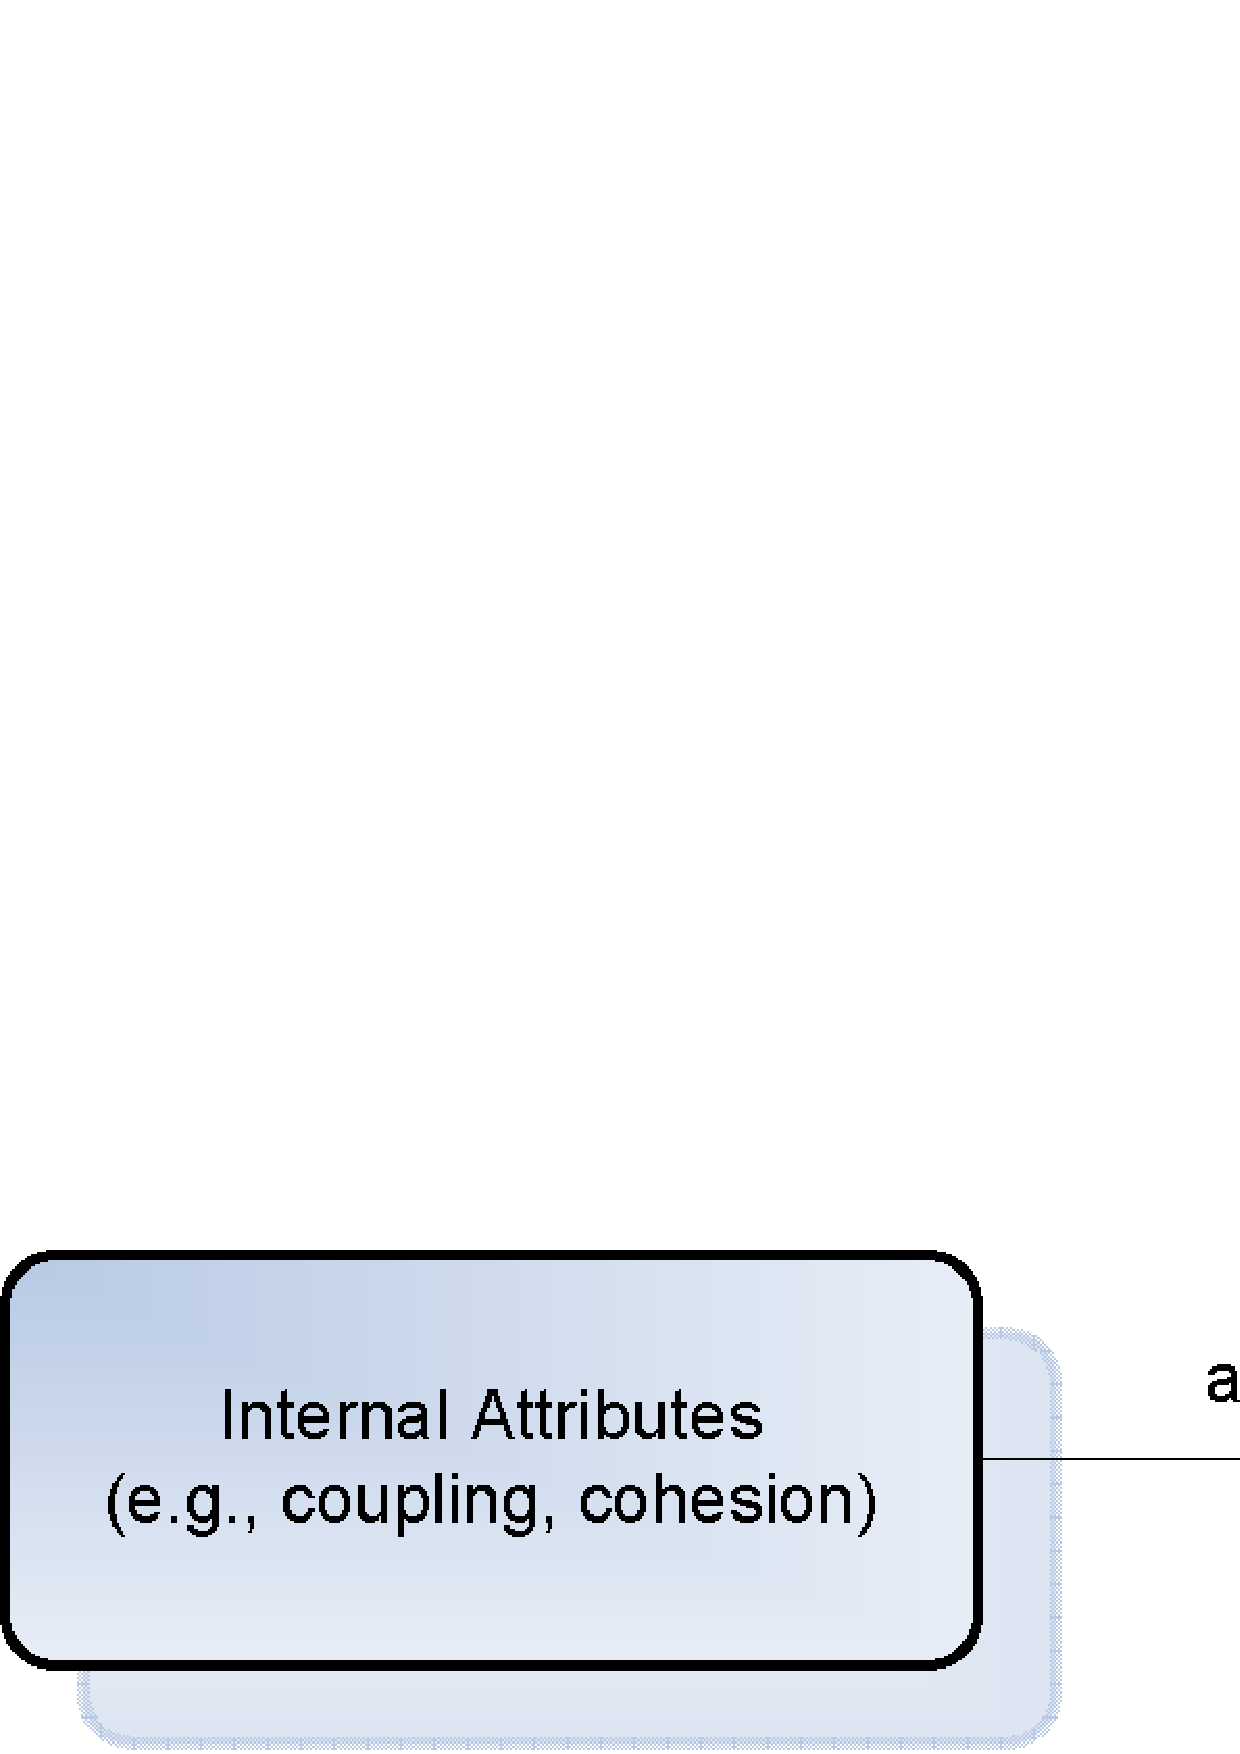
\includegraphics[width=1.00\textwidth]{figures/CognitiveComplexity}
  \caption{Cognitive Complexity Theory} 
  \label{fig:CognitiveComplexity}
\end{figure}

Software project telemetry facilitates validation of internal product metrics empirically. The fact that telemetry charts and reports juxtapose telemetry streams for the same time period, and that telemetry streams can be updated in real time, makes it easy to detect correlation between different metrics. For example, one may detect that an increase in code coupling is always accompanied by a jump in the number of open bugs. Though correlation is by no means causality, such empirically observed correlation does provide useful information when one tries to develop a hypothesis of causality. After the hypothesis is generated, such as lowing code complexity reduces the number of bugs, one can continue to use software project telemetry to either confirm or reject the hypothesis based on empirical evidence.


\subsubsection{External Validation}

In the experimental context, external validation refers to the extent to which the results generated in one setting can be expected to hold true in other settings. Software project telemetry process methodology employs cycles of process problem detection, improvement hypothesis generation, change implementation, and hypothesis validation to empirically guide project management and process improvement decision-making (see Section \ref{Telemetry:Process}). Since the cycles are executed within a project, it does not guarantee that a process improvement hypothesis validated in one project will also be valid in another project. External validation has to be performed in order to assess the applicability process improvement practice in other environment, such as in another project or another organization. Currently, the research of software project telemetry focuses on laying a common foundation for measurement machinery and process methodology. In the future, more research will be conducted to accumulate a repository of process improvement hypotheses that are validated on a wide basis.

\end{comment}

%%%%%%%%%%%%%%%%%%%%%%%%%%%%%%%%%%%%%%%%%%%%%%%%%%%%%%%%%%%%%%%%%%%%%%%%%%%%%%
%               E N D   O F   C O M M E N T
%%%%%%%%%%%%%%%%%%%%%%%%%%%%%%%%%%%%%%%%%%%%%%%%%%%%%%%%%%%%%%%%%%%%%%%%%%%%%%




%%%%%%%%%%%%%%%%%%%%%%%%%%%%%%%%%%%%%%%%%%%%%%%%%%%%%%%%%%%%%%%%%%%%%%%%%%%%%%
%%%%%%%%%%%%%%%%%%%%%%%%%%%%%%%%%%%%%%%%%%%%%%%%%%%%%%%%%%%%%%%%%%%%%%%%%%%%%%
\section{The Personal Software Process}  \label{RelatedWork:PSP}

The Personal Software Process (PSP\footnote{Both Personal Software Process and PSP are registered service marks of Carnegie Mellon University.}) \cite{Humphrey:1995, Humphrey:1996} is a self-improvement process for software developers, and a ground-breaking approach that adapts organizational-level software measurement and analysis techniques to the individual. 

The PSP provides both measurement machinery and process methodology. The primary goals of the PSP are to improve project estimation and quality assurance. The goals are pursued by observation-evaluation-modification cycles. Developers observe their performance by recording how they develop software. They record the amount of time they spend, the size of the work product, and the defects they made while developing software. At the end of each project, developers evaluate how they performed by conducting standard analyses on the metrics they collected. Based on project postmortems, developers gain insight into their development process, and modify it in an attempt to improve it. A new cycle starts with the modified developement process.

The original PSP proposed by Humphrey uses a manual approach, which is very tedious. For instance, every time a compilation error occurs, the developer has to stop his/her current work, and log on paper forms the details about the error. Though several studies \cite{Ferguson:1997, Hayes:1997, Khajenoori:1995} have shown that the PSP appears to help improve software development, the anecdotal evidence suggests that the overhead involved in manual data collection affects its adoption. For example, a report on a workshop of PSP instructors \cite{Borstler:2002} reveals that in one course of 78 students, 72 of them abandoned the PSP because they felt ``it would impose an excessively strict process on them and that the extra work would not pay off''. None of the remaining 6 students reported any perceived process improvements. Moreover, manual data collection is susceptible to bias (either deliberate or unconscious), error, omission, and delay. A study \cite{Johnson:1998} of the data collected in the PSP showed that there were significant issues of data quality, and the combination of data collection and analysis errors called into question the accuracy of manual PSP results. Humphrey, the author of PSP, also admits in his book \textit{a Discipline for Software Engineering} \cite{Humphrey:1995} that ``it would be nice to have a tool to automatically gather the PSP data''.

Tools, such as LEAP \cite{Moore:1999}, PSP Studio \cite{PspStudio:1997} and Software Process Dashboard \cite{PspDashboard:2000}, does exist to support the original manual PSP. These tools follow the same approach to user interaction by displaying dialog boxes where the user can log effort, size, and defect information. Though tool support lowers data collection overhead considerably, it turns out that the adoption of these tools is not satisfactory because of the requirement that the user constantly switch back and forth between doing work and telling the tool what work is being done \cite{Johnson:2001} \cite{Johnson:2003}. This chronic context switch appears to be a problem for most developers.

Software project telemetry uses sensors to collect metrics.\footnote{Sensor-based approach to metrics collection is pioneered in the Hackystat project \cite{Johnson:2003}, developed in Collaborative Software Development Lab (CSDL) of University of Hawaii. Hackystat is a framework that provides novel support for software measurement definition, validation, and software engineering experimentation. I have been on the core Hackystat development team since 2002, while doing software project telemetry related research. The reference implementation of software project telemetry mentioned in this paper is based on the Hackystat framework.}. Sensors are attached to software development tools, which monitor some form of state change in the project development environment. Sensors intend to collect metrics automatically and unobtrusively in order to keep data collection overhead sufficiently low, so that developers are not distracted from their primary tasks -- developing software products. Compared to manual and tool-based data collection, sensor-based approach not only automates metrics collection in an unobtrusive manner, but also eliminates the chronic context-switch overhead. Details about sensor data collection, as well as its restriction, are discussed in Section \ref{Telemetry:Data} of Chapter \ref{Chapter:Telemetry}.

As far as process methodology is concerned, the PSP uses observation-evaluation-modification cycles to improve software development process. One cycle corresponds to the life time of one project, and process improvement is based on comparison of different projects. This is essentially model-based cross-project comparison. The limitation is that it requires a historical database of finished projects. The PSP does not yield benefit unless such a database is accumulated first. For example, one of the practices of the PSP is to use statistical regression to predict project time based on planned project size. This requires sufficient number of data points with respect to time and size information of past projects. Even if the accumulation of a historical project database is not a problem, the PSP user still must make sure that the context of the current project is consistent with the contexts of the finished projects in the project database. Otherwise, the prediction process is like comparing apples to oranges. The context consistency problem will be discussed in detail Section \ref{RelatedWork:COCOMO} of this chapter, since all model-based approaches face the same limitation.

Similar to the PSP, software project telemetry uses cycles to improve software development process. The cycle includes process problem detection, hypothesis generation, change implementation, and hypothesis validation. The difference is that software project telemetry cycle does not correspond to the life time of a project. It involves much smaller time scale, and a single project can have multiple cycles. The idea behind software project telemetry is that comparison can be made between two different periods of the same project, instead of between two different projects, and the changes in the development process and their trends can be used as the basis for process improvement decision making. Since software project telemetry does not make model-based cross-project comparison, there is neither need to accumulate historical project database, nor necessity to ensure context consistency between different projects.







%%%%%%%%%%%%%%%%%%%%%%%%%%%%%%%%%%%%%%%%%%%%%%%%%%%%%%%%%%%%%%%%%%%%%%%%%%%%%%
%%%%%%%%%%%%%%%%%%%%%%%%%%%%%%%%%%%%%%%%%%%%%%%%%%%%%%%%%%%%%%%%%%%%%%%%%%%%%%
\section{The Constructive Cost Model} \label{RelatedWork:COCOMO}

The Constructive Cost Model (COCOMO) \cite{Cocomo:1981, Cocomo:2000} is a model for software project cost / effort estimation. It belongs to the branch of software engineering research called model-based process prediction. This section begins with the more general topic of model-based process prediction before going to the details of COCOMO.

The research in the area of model-based process prediction typically involves the following basic procedure: (1) collect a set of process and product metrics, such as size, effort, complexity, and defects, for a set of completed software projects, (2) generate a model to fit the observed data, (3) and claim that the model can be used to predict characteristics of future projects. For example, a model might predict that a future project of size \textit{S} will require \textit{E} person-months of effort; another model might predict that the future implementation of a module with complexity \textit{C} will be prone to defects with density \textit{D}. 

%Model-based process prediction is related to external validation of software product internal metrics (see Section \ref{RelatedWork:MetricsExternalValidation}), but with different focus. Model-based process prediction concerns more about predicting characteristics of a future project using existing metrics; while product internal metrics external validation concerns more about proving usefulness of a metric by showing its correlation to the properties of a project we care about.

Model-based process prediction can be compared to software project telemetry with respect to measurement machinery. The difference is that prediction in software project telemetry does not require the building of a model. Instead, it relies on changes in the development process and their trends to make short-term in-process predictions. The predictions made in software project telemetry and those made in model-based approaches tend to be of a different nature: model-based approaches tend to make end-point estimations (predictions for all phases of a software project as a whole), such as $X$ man-hours are needed to finish project $A$; while software project telemetry tend to make in-process predictions, such as the number of open bugs in system $B$ will continue to increase if system test coverage does not stop dropping.



%Software cost estimation usually involves the determination of one or more of the following estimates:
%\begin{itemize}
%  \item Development Effort (typically measured in person-months)
%  \item Project Duration (typically measured in calendar time)
%  \item Monetary Cost (typically measured in dollars)
%\end{itemize}
%
%Most cost estimation models first generate an effort estimate which is often measured in person-months of analysts, programmers and project managers. Then this effort estimation is converted to project duration and monetary cost. The conversion may not be trivial since project effort, duration and cost are usually not related to each other by simple transformation.
%
%Mainstream models use parametric estimation, which is based on statistical procedures that relate software development effort estimate to a number of factors. The general estimation formula is:
%\begin{equation}
%	Effort = f(X_1, X_2, ..., X_n)
%\end{equation}
%where \textit{Xi} denotes the factor that affects development effort. 

Since model-based process prediction researches follow similar approaches in model building and process prediction, COCOMO is used to illustrate how they work. COCOMO is chosen because it is one of the widely available and accepted models in the public domain.
%The Constructive Cost Model (COCOMO) \cite{Cocomo:1981, Cocomo:2000}
COCOMO is developed by Barry Boehm and his associates at University of Southern California.  The model estimates effort and schedule required to complete a software project. The COCOMO 81 was the original model published in the book \textit{Software Engineering Economics} \cite{Cocomo:1981}. It offers 3 levels of model with increasing detail and accuracy: \textit{basic}, \textit{intermediate}, and \textit{detailed}. COCOMO II \cite{Cocomo:2000} is an updated version of the original model to reflect the changes in software development practice. Like the first version, COCOMO II offers 3 levels, \textit{application composition}, \textit{early design}, and \textit{post-architecture}, to explicitly model the fact that uncertainty of effort and schedule estimates decrease through software project life cycle. 

%The primary input to the model is the estimated proejct size of the finished system. Size can be measure in lines of code, function points \cite{Albrecht:1983}, or object points \cite{Banker:1991, Banker:1994}.
%
%The application composition model is the simplest of all. It is used for rough order of magnitude estimation of costs on projects that use integrated computer aided software engineering (CASE) tools for rapid application development (RAD). It is based on object points \cite{Banker:1991} \cite{Banker:1994} which count the number of screens, reports and 3 GL language modules. Effort is modeled as a non-linear function of software size:
%  \begin{equation}
%    Effort = A * Size ^ B
%  \end{equation}
%
%The early design model and post-architecture model use the same approach to product sizing and scale factors to account for differences in hardware constraints, personnel quality and experience, use of modern tools and techniques, and other significant factors in software development projects. The early design model is a high-level model that can be used to explore architectural alternatives or incremental development strategies, while the post-architecture model is a detailed model that is typically used after the software architecture is defined and established. Both models have the same functional form. The only difference is that the post-architecture model uses more effort multipliers than the early design model.

The post-architecture model is used below to illustrate how COCOMO works. The estimation equations in the post-architectural model are:
  \begin{equation}
    PM = A * \prod_{i=1}^{17}EM_{i} * Size ^{(B + 0.01 * \sum_{i=1}^{5}SF_{i})}
  \end{equation}

  \begin{equation}
    TDEV = C * PM ^{(D + 0.002 * \sum_{i=1}^{5}SF_{i})}
  \end{equation}
where $PM$ is estimated effort in person-months. A person-month is the amount of time one person spends working on a software development project for one month. Note that this is in nominal terms, which does not take schedule compression or expansion into account\footnote{COCOMO II offers an effort multiplier $SCED$, which can be used to adjust for the effect of schedule compression or expansion.}. $Size$ is the primary input to the model. It is expressed in thousands of source lines of code (KSLOC). COCOMO II not only offers detailed rules on how to count lines of code, but also provides methods to covert other counting results, such as function points\footnote{Function point is a measure of program size independent of technology and programming language. The value of function point $FP$ is the product of unadjusted function points $UFP$ and technical correction factor $TCF$. Support for setting up function point analysis program is available from International Function Point User Group (http://www.ifpug.org).} \cite{Albrecht:1983} and object points \cite{Banker:1991, Banker:1994}, to lines of code. $TDEV$ is the amount of calendar time it will take to develop the software product. The average number of staff can be derived by dividing $TDEV$ from $PM$.

$A$, $B$, $C$, $D$, $SF_i$ and $EM_i$ are all constants in the model. $SF_i$ is called scale factor which influences effort exponentially. Scale factors are used to account for the relative economy or dis-economy of scale encountered for software projects of different sizes. $EM_i$ is called effort multiplier which influences effort multiplicatively. Effort multipliers are used to adjust for different product, project, platform and personnel factors in different software product development. Both effort multipliers and scale factors are defined by a set of rating levels (e.g. Very Low, Low, Nominal, High, etc.). 

Every few years, COCOMO team updates the model by supplying new calibration values for the constants to reflect latest change in software production practice in industry. For example COCOMO II 2000 post-architecture model calibration values were obtained by calibrating the model to the actual parameters and effort values for the 161 projects in the COCOMO II database at that time. These values represent the software industry average. COCOMO recommends its users to calibrate $A$, $B$, $C$ and $D$ to their local development environment in order to increase prediction accuracy of the model.

COCOMO enjoys wide acceptance in both academia and industry. Various extensions have been developed since the publication of the original model. These extensions include COQUALMO (Constructive Quality Model) \cite{COQUALMO:1999}, COCOTS (Constructive COTS Model) \cite{COCOTS:2000}, and CORADMO (Constructive Rapid Application Development Model) \cite{CORADMO:2001}. Commercial implementations include Costar from Softstart Systems \cite{Software:Costar}, Cost Xpert from Cost Xpert Group Incorporated \cite{Software:CostXpert}, and Estimate Professional from Software Productivity Center Incorporated \cite{Software:EstimateProfessional}. 



%\subsection{Relationship with Software Project Telemetry}

% [Find Reference] Other parametric models include Jensen Model, Checkpoint [Jones 96], PRICE-S, Softcost [Tausworthe 81], etc.

The basic idea behind COCOMO and other process prediction models is cross-project comparison. Unfortunately, there are a number of difficulties in adopting this method.
%it generally yields results not easily translated into practice. 

First, model-based process prediction assumes that the software organization has a relatively stable and repeatable development process. However, according to a Software Engineering Institute (SEI) survey of 542 software development organizations \cite{Peterson:1997}, 67\% of them are at CMM maturity level 1 - the lowest maturity level. By definition, the software processes at level 1 are \textit{ad hoc} and sometimes \textit{chaotic}, and they change as work changes. As a result, it is generally impossible to make predictions for organizations at this level. In other words, two-thirds of software organizations cannot benefit from model-based process predition, such as COCOMO.

Second, the prediction power of the models highly depends on how well model calibration is performed. This can be thought of as a context consistency problem. In order to use the model, practitioners must confirm that the set of projects used to calibrate the model are similar to the project they wish to predict. Otherwise, they must recalibrate the model using the data in the organization's historical project database. This involves replicating the model-building method within the practitioner's organization, with the risk that the organization may have already changed and the context of future projects may differ from those in the historical project database. 

Lastly, model-based process predictions are primarily designed to be used at very early stage of a software project, or even before a project actually starts. Therefore, they tend to make end-point estimations (i.e. the prediction is made for all phases of the project as a whole). For example, COCOMO estimates that 586 person-months are required to develop a software with estimated size of 100 KSLOC\footnote{Suppose all scale factors and effort multipliers take the rating of \textit{nominal}. Using COCOMO II 1997 calibration data, the estimation equation is $PM = 2.94 * Size ^ {1.15}$.}. But when 300 person-months have been spent writing 60 KSLOC, the model does not give any indication whether the project will still be on-target or not. One will know the answer only after the entire project is finished, but everything will be too late at that time. In other words, end-point estimations have no in-process control capabilities.

Software project telemetry avoids the above-mentioned difficulties by shifting the focus of process prediction. It makes no attempt to build a rigorous cross-project comparison model in order to make a prediction before the project starts. Instead, it employs a more agile approach to compare software processes in different periods within the same project. It relies on the changes in the development process, as well as the trends of the changes, to make short-term predictions for the purpose of in-process project management. 





%Parametric models usually cannot be used off-the-shelf. They often require calibration to the local software development environment and development process. Calibration is especially important when the context of model application (e.g. application domain, organization size, available resources) is different from the original context in which the model was originally built. Once calibrated to relevant project data, the calibrated parameters can be used to understand the relative strengths of different factors, and provide direction for software organizations to improve their development process and reduce cost.
% 
%Calibration is a requirement for all estimation models. It is not an easy task. It requires a historical database of with sufficient amount of metrics from previous projects. Even if such a database has been accumulated, historical data may have limited value if projects are too diverse or poorly defined for sensible comparison. In general, calibration is well-beyond the capability of any single software development organization except for some largest corporations. 


%\begin{figure}[tbp]
%  \includegraphics[width=1.00\textwidth]{figures/CMM-Distribution}
%  \caption{CMM Process Maturity Distribution \cite{Peterson:1997}} 
%  \label{fig:CMM-Distribution}
%\end{figure}
%
%Apart from difficulty in calibration, parametric models face several other difficulties.
%\begin{itemize}
%	\item Strictly speaking, using of parametric models may not theoretically sound in the field of software engineering. Parametric models are generated from data sets with distributions determined by a finite number of real parameters. They may only be used under certain rather limiting conditions. For example, the data distribution must be normal and continuous, and samples should be randomly drawn from a single population, which is often not the case in calibration data. Inappropriate use of parametric techniques will lead to erroneous results. \textbf{[Lost reference]}
%
%  \item	The basic idea behind all estimation models is repeatable software development process. However 67\% of software development organizations are at CMM process maturity level 1 \cite{Peterson:1997} (Table \ref{fig:CMM-Distribution}). By definition the software processes at level 1 are \textit{ad hoc} and sometimes \textit{chaotic}, and they change as work changes. As a result it's generally impossible to predict schedules and budgets for organizations at this level. Therefore, estimation models are useless to the majority of software development organizations.  
%
%  \item Most cost estimation models cannot deal with small project satisfactorily. One cause is the construction of the model themselves. Some models, such as SLIM, are macro models, and they are only designed to handle large projects. Another cause is the data used in calibrating the model. Prediction for small projects requires extrapolation of the model, which results in large error variance.
%  
%  \item \textcolor{red}{An important responsibility of software project manager is tracking the actual size, effort, budget, and schedule against the estimates in the approved plan. However, the size on the estimate chart is finishing point of project of different size, not the size at different stage of software development. So no tracking capability.}
% 	
%\end{itemize}











%\subsection{Putnam Model and SLIM}
%
%The Putnam model \cite{Putnam:1978} is one of the first parametric models. It is based on a negative exponential curve called the \textit{Rayleigh-Norden} effort curve, which indicates the man-power distribution over time during the software life cycle. The central part of the model is the \textit{software equation}:
%  \begin{equation}
%    Size = Env * {Effort ^ {\frac{1}{3}}} * {T_{d} ^ {\frac{4}{3}}}
%  \end{equation}
%where \textit{Td} is the software delivery time. \textit{Env} is the constant in the model, which represents the environment factors that determine the development capability. The constant can be calibrated from historical data using the software equation. \textit{Size} is measured in lines of code, and \textit{Effort} is measured in person-year.
%
%The Software Life Cycle Model (SLIM) \cite{SLIM} from Quantitative Software Measurement (QSM\footnote{http://www.qsm.com}) is a commercial version of the Putnam model \cite{Putnam:1978}. QSM is a consulting company supplying products and services that enables software development organizations to measure, estimate and control projects.
%
%The SLIM effort estimation equation is:
%  \begin{equation}
%    Effort = (12^5*B)*  (\frac{SLOC}{P})^3  *  \frac{1}{Schedule^4}
%  \end{equation}
%where \textit{P} is the productivity parameter, and \textit{B} is the special skill factor. The equation is derived from data of over 6300 completed software projects collected by Larry Putman and his associates at QSM. The model indicates that there is effort schedule trade-off.
%
%SLIM bad (1) Estimates are extremely sensitive to the technology factor (2) Not suitable for small projecs. (Actually, models cannot be used to extrapolate.) Compared to SLIM or other estimation models, COCOMO has two major advantages: Constructiveness, Open Source. Being in the public domain is its disadvantage as well. The internal equations and parameter values are fully-available.












%%%%%%%%%%%%%%%%%%%%%%%%%%%%%%%%%%%%%%%%%%%%%%%%%%%%%%%%%%%%%%%%%%%%%%%%%%%%%%
%%%%%%%%%%%%%%%%%%%%%%%%%%%%%%%%%%%%%%%%%%%%%%%%%%%%%%%%%%%%%%%%%%%%%%%%%%%%%%
\section{The Goal-Question-Metric Paradigm} \label{RelatedWork:GQM}

%\begin{quote}
%  \textit{Data should be collected with a clear purpose in mind. Not only a clear purpose but a clear idea as to the precise way in which they will be analyzed so as to yield the desired information.}  \begin{flushright}\textit{--- Moroney, 1950}\end{flushright}
%\end{quote}

While software project telemetry requires telemetry streams to be used to monitor the development process of a software project, it never specifies what telemetry streams should be used. This is actually not a deficiency of software project telemetry. Because different projects and different organizations have different development environment and different project goals, it is impossible to prescribe the required telemetry streams. 

Many organizations opportunistically collect metrics based on what is easy to collect. If software project telemetry is introduced to these organization, they would naturally extend the bottom-up approach by generating telemetry steams based on available metrics. While bottom-up approach sometimes works, it is best to collect data and use software project telemetry in a top-down fashion with a clear purpose in mind. 

The Goal-Question-Metric paradigm (GQM) \cite{Basili:1988, Basili:1992} has no measurement machinery, but it provides a top-down, goal-oriented process methodology that can be used in conjunction with software project telemetry. In GQM, software measurement is driven by high level goals. Usually business goals of an organization are formed first and then translated into improvement goals of software development, which, in turn, are translated into measurement goals. A metrics program is used to fulfill the measurement goals. Based on the measurement outcome, the organization can generate hypotheses and make proper decisions in order to reach the improvement goals and finally the business goals.

GQM offers a top-down method to translate high level measurement goals into questions that need to be answered in order to reach the goals. Based on the questions a set of relevant metrics can be identified and collected, which provide answers to those questions. This leads to a tree-structured graph depicted in Figure \ref{fig:gqm}.

\begin{figure}[tbp]
	\centering
		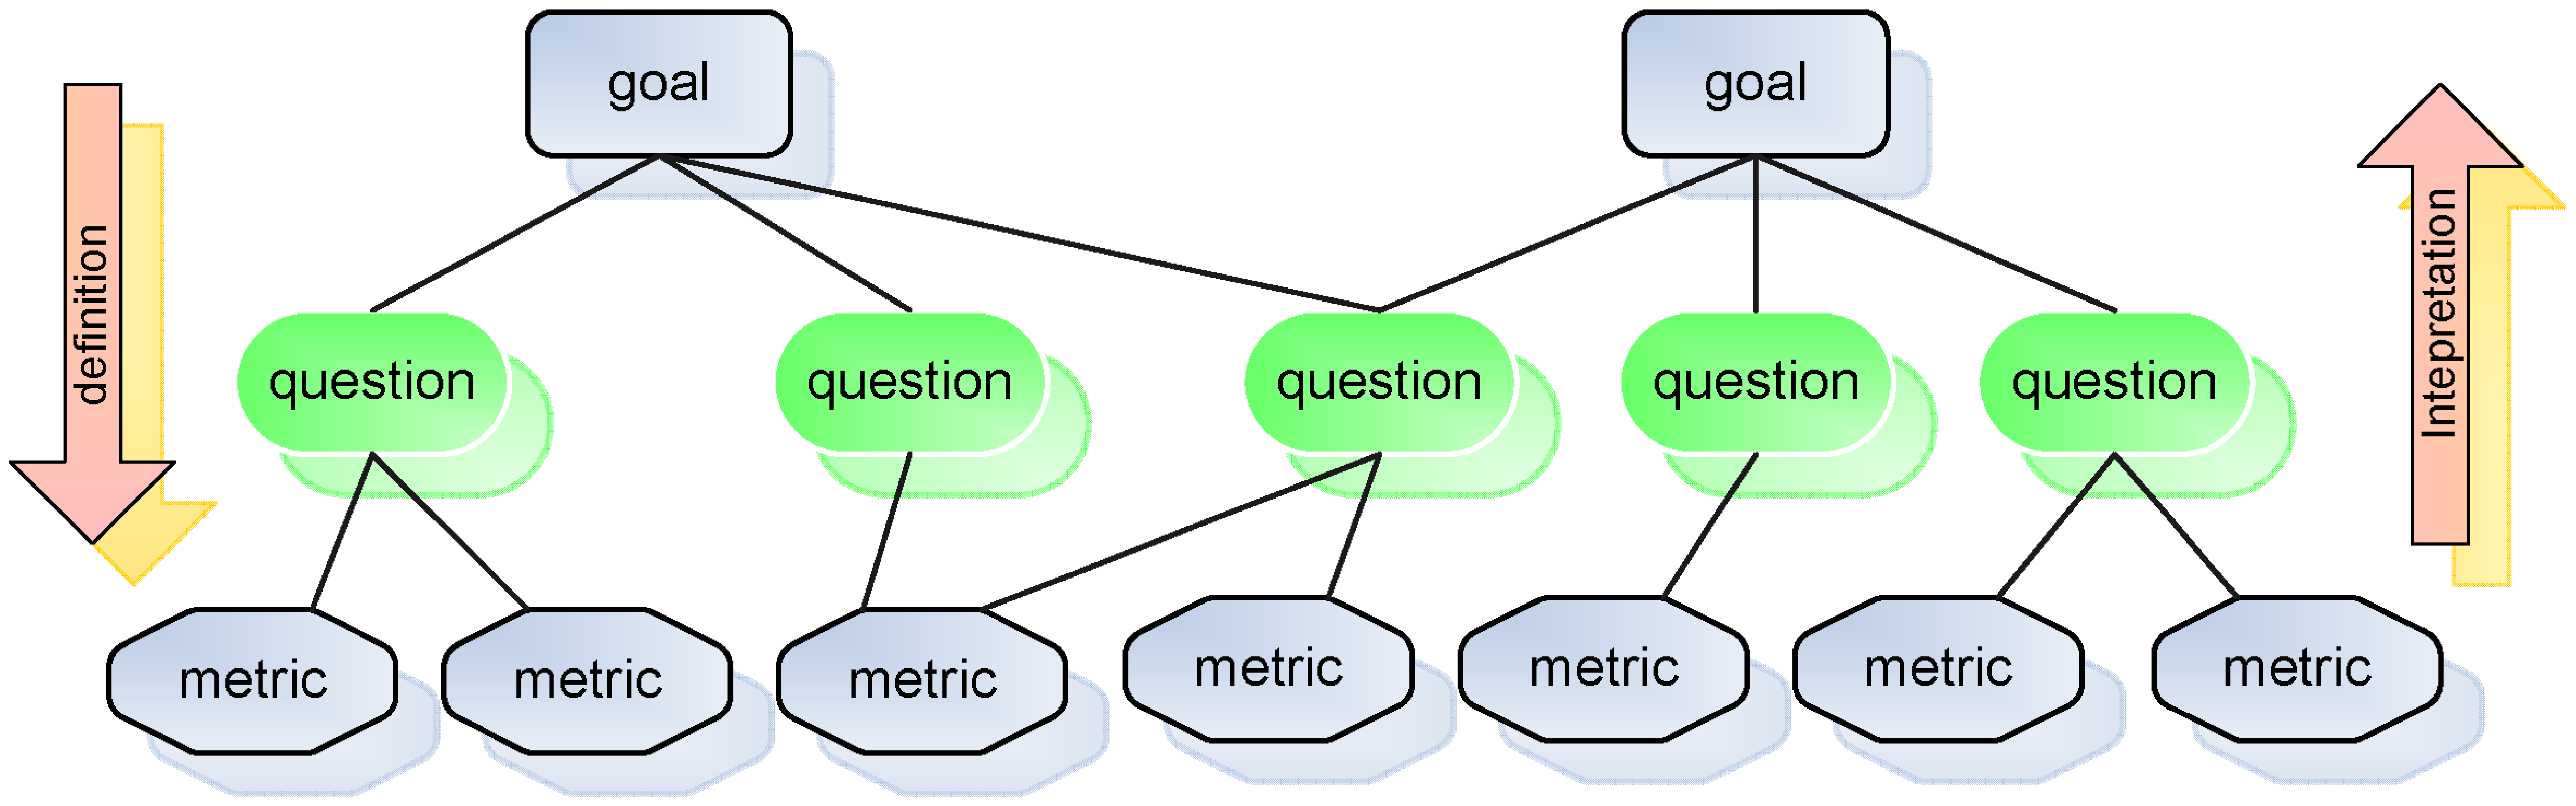
\includegraphics[width=1.00\textwidth]{figures/GQM}
		\caption{Goal-Question-Metric Paradigm}
	\label{fig:gqm}
\end{figure}

%GQM measurement goal is stated in 5 dimensions:
%\begin{itemize}
%	\item \textit{Object of Study} --- The entity or entities that should be studied, e.g. a software specification, a testing process.
%	\item \textit{Purpose} --- The reason for the measurement. 
%	\item \textit{Quality Focus} --- The attributes or attributes that should be studied.
%	\item \textit{Point of View} --- The viewpoint of the person or the organization from which the measurement is carried out.
%	\item \textit{Environment} --- The context in which measurement is carried out.
%\end{itemize}

GQM measurement goal is stated in 5 dimensions: \textit{study object}, \textit{purpose}, \textit{quality focus}, \textit{view point}, and \textit{environment}. A concrete example can be found in \cite{Solingen:1998, Solingen:1999}. The authors studied causes and effects of interrupts on software development work, and their measurement goal was ``\textit{analyze} interrupts and their effects \textit{for the purpose of} understanding \textit{with respect to} impact on schedule and the cost-benefit of interrupts \textit{from the viewpoint of} project team \textit{in the context of} project $X$''.

%The authors generated the following questions to operationalize the goal:
%	*What is the influence of interrupts on the work that was interrupted?
%	*What factors influence treatment and effort for handling an interrupt?
%	*Is prevention of interrupts possible?
%
%After that, metrics were identified and collected in order to answer the questions. Some of the metrics used by the authors were:
%	*Number of interrupts for current work.
%	*Number of interrupts for non-current work.
%	*Number of interrupts that are treated immediately.
%	*Number of interrupts that are planned.
%	*Number of interrupts per day.
%	
%	
%The interpretation of the metrics proceeds bottom-up, from the metrics to the questions, and finally to top level business goals. Based on the metric data collected, it was discovered that interrupts accounted for about 20\% of total time of the software organization under the study. The result prompted actions to encourage eletronic communication, such as emails, among developers instead of face-to-face communication.

GQM is well-known. Case studies of successful experience abound \cite{Basili:1996, Latum:1998, Fuggetta:1998}. The key to the success of GQM implementation appears to be the establishment of well-defined measurement goals and the derivation of software metrics that can be used to provide useful information to meet the goals. 

The main drawback of GQM paradigm is the lack of attention to the actual measurement process. Metrics collection, interpretation and analysis are not a part of the paradigm. Implicitly, GQM assumes that once all required metrics are identified, the rest steps (metrics collection and analysis) would be easy.

However, the drawback can be overcome by using GQM in conjunction with software project telemetry. When used together, they reinforce each other: GQM defines useful metrics and telemetry streams, and relates them to software organization's business, project, product, and process goals; while software project telemetry provides an automated infrastructure for metrics collection and analysis, as well as an in-process, empirically-guided methodology for process improvement. For example, ``continuous GQM'' tries to implement GQM in an automated way in which data is collected, analyzed, and presented automatically with minimal human effort \cite{Lofi:2005}.



%%%%%%%%%%%%%%%%%%%%%%%%%%%%%%%%%%%%%%%%%%%%%%%%%%%%%%%%%%%%%%%%%%%%%%%%%%%%%%
%%%%%%%%%%%%%%%%%%%%%%%%%%%%%%%%%%%%%%%%%%%%%%%%%%%%%%%%%%%%%%%%%%%%%%%%%%%%%%
\section{The Software Capability Maturity Model}  \label{RelatedWork:CMM}

The Software Capability Maturity Model (CMM) \cite{Paulk:1993, SEI:1995} is a process maturity framework developed by Software Engineering Institute (SEI). Other similar frameworks include ISO 9001 \cite{ISO9001:1987} and SPICE and ISO/IEC 15504 \cite{ISO:1998, Eman:1998}. They share common properties, such as using metrics as means to help software organizations improve their development process, and to assess their capabilities. In these approaches, an externally defined reference framework is used to prescribe the activities, methodologies and practices a software organization should implement. The implicit assumption is that the prescribed processes are needed by most organizations in order to deliver high quality software in a repeatable and controllable manner, and a mature software development process will deliver high quality software products on time and within budget. Process assessment is used to compare organizational processes with the reference framework, which serves as an effective driver for process improvement. The assessment can be done by the software organization itself, by the second party, or by an independent third party. Based on the assessment results, organizations can find directions for process improvement.

Software project telemetry is closely related to process maturity. On one hand, higher process maturity offers greater visibility into development activities. Since we can only measure what is visible in a process, higher process maturity means more telemetry streams can be generated and monitored. The process maturity scales offer a convenient context for determining what telemetry streams to use first, and how to plan software project telemetry program so that it grows to embrace additional aspects of development and management. On the other hand, software project telemetry offers a methodology for process improvement based on quantitative feedback from existing development processes. It is especially helpful for software organizations to achieve high process maturity levels where quantitative measurement is mandated, such as CMM level 4 or 5.


%The Software Capability Maturity Model (CMM) \cite{Paulk:1993, SEI:1995} 

The following discussion will focus on CMM to illustrate how a maturity framework works, since most maturity frameworks work in similar ways.

The goal of CMM is to determine whether a software development organization has a sound management infrastructure, and to assess its level of competence in building high quality software products. CMM is a staged model, which provides a set of requirements that software development organizations can use to set up software processes to control software product development. It ranks a software organization's process capability on a maturity level from 1 (lowest) to 5 (highest):

\begin{enumerate}
  \item \textit{Initial Stage:} The software process at this level is characterized as \textit{ad hoc} and sometimes \textit{chaotic}. Success of software projects depends on competence and commitment of individual developers. Few software processes are defined, and they change as work progresses. As a result, schedules, budgets and quality are generally unpredictable.
  \item \textit{Repeatable Stage:} Basic project management processes are in place. Software organizations at this level have controls over software requirements, project planning and tracking, configuration management, quality assurance and subcontractor management. They are able to track project cost and schedule, and they can repeat earlier successes on projects with similar applications.
  \item \textit{Defined Stage:} The software processes for both management and engineering activities are documented, standardized and integrated into a standard software process for the whole organization. All projects use an approved, tailored version of the organization's standard software process to develop and maintain software.
  \item \textit{Managed Stage:} Detailed measurement programs are in place to assess software development processes and product quality. Both software process and products are quantitatively understood and controlled. Software organizations at this level are able to tailor development processes to specific needs with predictable outcomes.
  \item \textit{Optimizing Stage:} Continuous process improvement is enabled by quantitative feedback from software development processes and from piloting innovative ideas and technologies.
\end{enumerate}

Each maturity level is associated with a number of processes that an organization must implement. These processes are grouped into key process areas (KPA). Each KPA has a set of goals, capabilities, key practices, as well as measurements and verification practices. There are a total of 52 goals and 150 key practices. Some are related to setting up basic project management controls; some are aimed at establishing an infrastructure that institutionalizes effective software engineering and management processes across projects; while the rest are focused on performing a well-defined engineering process that integrates all software engineering activities to produce correct, consistent software products effectively and efficiently. The maturity level of a software organization is determined by its demonstrated capability in the key process areas associated with that level. Table \ref{table:CMM-KPA} lists CMM levels and their associated key process areas.

\begin{table}[tbp]
	\centering
		\begin{tabular}{|p{0.25\textwidth}|p{0.65\textwidth}|} 
		  \hline
			\textbf{CMM Levels} & \textbf{Key Process Areas} \\
			% Level 1
			\hline 
			\textit{Level 1 -- Initial} & None. \\
			% Level 2
			\hline
			\textit{Level 2 -- Repeatable} & Requirements Management, Software Project Planning, Software Project Tracking and Oversight, Software Subcontract Management, Software Quality Assurance, Software Configuration Management. \\
			% Level 3
			\hline
			\textit{Level 3 -- Defined} &  Organization Process Focus, Organization Process Definition, Training Program, Integrated Software Management, Software Product
Engineering, Intergroup Coordination, Peer Reviews. \\
			% Level 4
			\hline
			\textit{Level 4 -- Managed} & Quantitative Process Management, Software Quality Management. \\
			\hline
			% Level 5 
			\textit{Level 5 -- Optimizing} & Defect Prevention, Technology Change Management, Process Change Management. \\
			\hline
		\end{tabular}
	\caption{CMM Levels and Key Process Areas}
	\label{table:CMM-KPA}
\end{table}

CMM has received much attention in both academia and industry. Quite a few positive experiences have been reported in the literature \cite{Humphrey:1991, Dion:1993, Daskalantonakis:1994, Diaz:1997}. For example, Humphrey \textit{et. al. }\cite{Humphrey:1991} reported a software process improvement program at Hughes Aircraft with estimated annual saving at about \$2 million.



%\subsection{ISO 9001}
%
%ISO 9001 \cite{ISO9001:1987} is an international standard for quality management and assurance that can be applied to organizations that design, develop, produce, install and service products. It is made up of 20 sets of quality system requirements. ISO 9001 does not assign maturity levels to software organizations, instead it only addresses the minimum requirements for an acceptable quality system.
%
%Paulk \cite{Paulk:1995} compared ISO 9001 with SEI Software Capability Maturity Model. He concluded that an ISO 9001 compliant organization would be somewhere between level 1 and level 3 of the CMM, and conversely a CMM level 2 or 3 organization would probably be considered ISO 9001 compliant.
%
%
%
%\subsection{SPICE and ISO/IEC 15504}
%
%Software Process Improvement and Capability Determination (SPICE), which led to ISO/IEC 15504 \cite{ISO:1998, Eman:1998}, is an international standard for software process assessment. It is based on CMM, but aims to consolidate the existing assessment frameworks. It defines processes essential to good software engineering practice. Base practices, which contain the minimum compliance requirements, are specified for each process. During assessment, an adequacy rating is given to each base practice. Possible adequacy ratings are \textit{fully, largely, partially or none}. They indicate how compliant an organization is to the practice in question. The maturity levels are listed in Table \ref{table:ISO-15504}.
%
%\begin{table}[tbp]
%	\centering
%		\begin{tabular}{|p{0.25\textwidth}|p{0.65\textwidth}|} 
%		  \hline
%			\textbf{ISO/IEC 15504 Levels} & \textbf{Description} \\
%			% Level 0
%			\hline 
%			\textit{Level 0 -- Incomplete} & There is almost no process and no identifiable work products of the process. \\
%			% Level 1
%			\hline
%			\textit{Level 1 -- Performed} & The purpose of the process is generally achieved, but the achievement may not be rigorously planned and tracked. \\ 
%			% Level 2
%			\hline
%			\textit{Level 2 -- Managed} & The process delivers work products of acceptable quality within defined timescales. Performance according to specified procedures is planned and tracked. \\
%			% Level 3
%			\hline
%			\textit{Level 3 -- Established} & The process is performed and managed using a defined process based on good software engineering principles. \\
%			% Level 4
%			\hline
%			\textit{Level 4 -- Predictable} & The defined process is performed consistently in practice within defined control limits. \\ 
%			% Level 5 
%			\hline
%			\textit{Level 5 -- Optimizing} & Continuous process monitoring is enabled by obtaining quantitative feedback. Process improvement is achieved by analysis of the feedback. \\
%			\hline
%		\end{tabular}
%	\caption{ISO/IEC 15504 Maturity Levels}
%	\label{table:ISO-15504}
%\end{table}
%
%There are not many differences between SEI CMM and ISO/IEC 15504, except the following:
%\begin{itemize}
%	\item ISO/IEC 15504 is a continuous model. As opposed to the staged model (such as CMM) where processes are attached to each maturity level, ISO/IEC 15504 measures the maturity of individual processes instead of the maturity of an entire organization.
%	\item ISO/IEC 15504 includes a framework for conducting assessments, as well as guidelines for the use of the framework in both self-assessment (for process improvement) and process capability determination.
%\end{itemize}
 
 
 


%\subsection{Relationship with Software Project Telemetry}

CMM makes use of software metrics to help software organizations improve their development process. It prescribes that in all key process areas measurement should be taken to determine the status of development activities. However, it does not prescribe explicitly how the measurement processes themselves should be implemented. In fact, Humphrey is aware of the difficulty of implementing a measurement program in a software organization. He mentioned in \cite{SEI:1995} that ``the greatest potential problem with the managed process (CMM level 4) is the cost of gathering data. There are an enormous number of potentially valuable measures of the software process, but such data is expensive to gather and to maintain.''.
 
Software project telemetry is a nice complement to the void left by CMM. It provides not only an automatic and unobtrusive way of gathering process data, but also a methodology of using quantitative data to analyze and modify software development process in order to prevent problems and improve efficiency. It is especially helpful to software organizations at high process maturity levels, such as CMM level 4 or 5.

CMM is useful to software project telemetry too. CMM maturity levels provide a convenient context for determining what telemetry streams to use first, and how to plan software project telemetry program so that it grows to embrace additional aspects of development and management. Indeed, several authors have studied the relationship between software measurement and process maturity. For example, Table \ref{table:Maturity-Measurement} lists Pfleeger and McGowan's recommendation of collecting different measures depending on a software organization's maturity level \cite{Pfleeger:1990}.

\begin{table}[tbp]
	\centering
%		\begin{tabular}{|p{7cm}|p{7cm}|}
		\begin{tabular}{|p{0.45\textwidth}|p{0.45\textwidth}|}
			\hline
			\textbf{CMM Maturity Level} & \textbf{What to Measure} \\
			\hline 
			\textit{Level 1 -- Initial: ad hoc} & baseline \\
			\hline 
			\textit{Level 2 -- Repeatable: process dependent on individual} & project \\
			\hline 
			\textit{Level 3 -- Defined: process defined and institutionalized} & product \\
			\hline 
			\textit{Level 4 -- Managed: process measured quantitatively} & process and feedback for control \\
			\hline 
			\textit{Level 5 -- Optimizing: continuing improvement based on measurement} & process and feedback for changing process \\
			\hline		
		\end{tabular}
	\caption{Process Maturity and Measurement}
	\label{table:Maturity-Measurement}
\end{table}







%Pfleeger 1995 \cite{Pfleeger:1995} presented a combinational approach to software measurement programs. The GQM paradigm is used to derive high level goals, while the CMM is used to decide what metrics to collect. As the software organization's  process matures a more comprehensive set of metrics can be measured. Hetzel 1993 \cite{Hetzel:1993} recommended the collection of a basic set of metrics for every project at all time. The reason behind it is that these basic metrics could stimulate questions and provide insights about the software products and their development processes.






%%%%%%%%%%%%%%%%%%%%%%%%%%%%%%%%%%%%%%%%%%%%%%%%%%%%%%%%%%%%%%%%%%%%%%%%%%%%%%
%%%%%%%%%%%%%%%%%%%%%%%%%%%%%%%%%%%%%%%%%%%%%%%%%%%%%%%%%%%%%%%%%%%%%%%%%%%%%%
%\section{Process Modeling}  \label{RelatedWork:ProcessReasearch}
%
%It is widely behieved that having a structured approach is very important for developing software products efficiently and effectively. A \textit{software process} is such a structured approach that describes how an organization develops and/or maintains a software system. It includes the people, machines, resources, tools, and artifacts in producing the software system. 
%
%A \textit{process model} is the formal description of the intended behavior of the process. It is an abstraction of a particular development approach, and the purpose is to reduce complexity of understanding of software process by removing unnecessary details. Process modeling includes both formal modeling and canonical modeling. Formal modeling uses the formulation of languages and paradigms to describe software processes in a mathematically unambiguous way. Paradigms used include programming \cite{Sutton:1995}, state machines \cite{Kellner:1991}, Petri nets \cite{Bandinelli:1993}, rule-based system \cite{Barghouti:1991} and planning \cite{Huff:1989}. Canonical models, on the other hand, tend not to be very specific. They only attempt to give a framework for more specific software development activities: requirement specification, design, implementation, verification and validation (testing and inspection). Examples of canonical models are the waterfall model, the spiral model, the ``cleanroom'' process \cite{Pressman:1992}, and the Rational unified process \cite{Software:RUP}. Some canonical models involve only specific sub-processes. Code inspection is perhaps the most studied one.
%
%Other researches in this field include process discovery and validation \cite{Cook:1996}. Process discovery is the act of devising a suitable model of a process execution, while process validation is the act of determining the level of correspondence between an executing process and a process model.
%
%\textit{Software project telemetry} is not directly related to process modeling, in the sense that it is not designed to assist discovering process model, or checking conformance between the model and the actual process. However, it can be used to manifest the results of executing a process model, and is good for comparing different process models. For example, extreme programming \cite{Beck:2000} advocates test-driven design. \textit{Software project telemetry} cannot detect whether a developer is actually doing test-driven design or not. However, once you know who is adopting the technique and who is not, you can use telemetry streams to compare process performance results, and answer questions such as whether test-driven design indeed results in more elegant design, less coding effort, and less bugs.
 

%It's often useful to structure a process  model using different views. Each view is an essential perspective that must be understood, defined, and managed. Ideally, when combined, these perspectives will produce an integrated, consistent, and complete process model.
%
%Three basic views are proposed by Humphrey  so9 [sec 13.11]: the state view, the organizational view, and the control view. The state view covers the various stages of product development. This includes both tasks and product states relating to design, coding, and testing. The organizational view of a software process model addresses the social aspect of development, which includes factors relating to communication and coordination, key roles and responsibilities, and motivation. The control view of a software process model focuses on direction. It deals with mechanisms for guiding development, which includes planning, approval, data gathering, support, and reporting.

%[Sommerville, I., Kotonya, G., Viller, S., Sawyer, P., Process Viewpoints, Procs. of the 4th European Workshop on Software Process Technology, Noordwijkerhout, The Netherlands, April 1995, ed. W. Sch�fer, LNCS 913, Springer-Verlag, Germany, 1995, pp. 2-8. http://citeseer.ist.psu.edu/3336.html] Quote: A process view point is an encapsulated process description which includes associated process models, which incorporate questions about process and potential process improvement. The questions can be:
%\begin{itemize}
%	\item \textit{Exploratory Questions:} These are intended to discover information about the process which is being studied. The answers to these questions influence the process models associated with a viewpoint. An example would be ``what mechanisms are incorporated int he process to monitor the costs of project activities.''
%	\item \textit{Improvement Questions:} These are intended to discover what is required to effect improvement in process. The answers to these questions should help identify process revisions. An example would be ``how can we reduce the time required to review documents''.
%\end{itemize}











%\subsection{Summary}
%
%
% Others include Bootstrap (Haase, Messnarz, Koch, Kugler and Decrinis 1994), largely based on CMM.
%
%All reference frameworks include measurement as means to help software organizations to improve their development process. For example CMM prescribes that in all key process areas measurements should be taken to determine the status of the activities. However, none of the reference frameworks prescribe explicitly how the measurement processes themselves should be implemented. 
%
%Standard-based frameworks face similar criticism, Software Capability Maturity Model will be used below to illustrate the criticisms they are facing:
%\begin{itemize}
%	\item \textit{Lack of a formal theoretical basis} --- It's a \textit{made-up} model, which describes an ideal organization that did not exist at the time the model was published. Whether the model indeed contains all activities needed by a mature software development organization is unknown.
%	
%	\item \textit{Construct validity issues} --- What is software process capability? Is it a concept similar to IQ? What's the nature of it? Does it really exist? Whether it can be measured? None of these questions are answered in CMM.
%	
%	\item \textit{Economic and cost effectiveness issues} --- How can an software development organization justify the costs involved in CMM-based improvement programs? Herbsleb, et al. \cite{Herbsleb:1997} found that it took on average two years per level for a software development organization to get from CMM level 1 to level 3, and that the cost ranged from \$500 to \$2000 per employee per year. Though ROI as high as 7.7 to 1 has been reported by Diaz and Sligo \cite{Diaz:1997}, question still remains whether all process improvement programs are that successful. 	
%
%\end{itemize}









%%%%%%%%%%%%%%%%%%%%%%%%%%%%%%%%%%%%%%%%%%%%%%%%%%%%%%%%%%%%%%%%%%%%%%%%%%%%%%
%%%%%%%%%%%%%%%%%%%%%%%%%%%%%%%%%%%%%%%%%%%%%%%%%%%%%%%%%%%%%%%%%%%%%%%%%%%%%%
%\section{Statistical Process Control}
%
%
%[Criticism for statical process control, Ould commenting on CMM] Ould (1996) criticizes the use of statistical analysis of the performance of the processes in use. He claims that treating software development as a manufacturing activity is an unhelpful demand, because it is not a manufacturing process, but an intellectual and sociological activity prone to many changes. Such changes include changes in the type  of work being done, changes in the technologies to be used, changes in staff or recruitment policy, etc. Thus, according to Ould, using statistical process control is neither appropriate nor necessary for defect prevention and process improvement.







%%%%%%%%%%%%%%%%%%%%%%%%%%%%%%%%%%%%%%%%%%%%%%%%%%%%%%%%%%%%
%
%       ***************   END   *****************
%
%%%%%%%%%%%%%%%%%%%%%%%%%%%%%%%%%%%%%%%%%%%%%%%%%%%%%%%%%%%%


\section{Summary}  \label{RelatedWork:Summary}

This chapter compares and contrasts software project telemetry to other metrics-based approaches. The Personal Software Process suffers from chronic metrics collection and analysis overhead. The Constructive cost model not only assumes that software development process is stable and thus predictable but also requires calibration. The Goal-Question-Metric Paradigm offers a high-level abstract process methodology but lacks attention to the actual measurement process. The Software Capability Maturity Model prescribes that measurement be taken to assess the status of development activities but does not specify how the measurement process should be implemented. Software project telemetry addresses these limitations through automated metrics collection and intuitive visual metrics analysis for in-process empirically-guided project management and process improvement. The next chapter details an implementation of software project telemetry.


%Software project telemetry consists of 2 related components: measurement machinery and process methodology. Existing approaches may contain only one of the components. The comparison made in this chapter is summarized in Table \ref{table:Process-Approaches-Classification}.
%
%\begin{table}[tbp]
%	\centering 
%		\begin{tabular}{|l|c|c|} 
%			\hline
%			\textbf{Approaches} & \textbf{Measurement Machinery} & \textbf{Process Methodology} \\
%			\hline
%			\textit{PSP} & \textit{X} & \textit{X} \\
%			\hline
%		  \textit{COCOMO} & \textit{X} & \textit{-} \\
%			\hline
%			\textit{GQM} & \textit{-} & \textit{X} \\
%			\hline
%			\textit{CMM} & \textit{-} & \textit{X} \\
%			\hline
%		\end{tabular}
%	\caption{Software Project Telemetry v.s. Other Approaches}
%	\label{table:Process-Approaches-Classification}
%\end{table}























%\textcolor{red}{[rewrite]}
%
%Mature software development process bring benefits to software development organizations, such as on-time within-budget delivery of high quality software products, improved predictability and productivity. Different perspectives on software development process improvement have been discussed in this chapter: goal-based, standard-based and model-based.
%
%Goal-based process improvement approaches mainly consists of measurement methodologies driven by high level business goals. Metrics are used to deliver the necessary information to make decisions in order to improve software development process.
%
%In standard-based process improvement approaches, processes and activities required for high quality software development are prescribed by external reference frameworks, and process assessments are used to find direction for improvement.
%
%In model-based process improvement approaches, software development costs are analyzed using mathematical formulas linking them with metrics. The calibrated parameters of the models are used to understand the relative impact of different factors, and provide direction for process improvement and cost reduction.
%
%Software metrics collection and analysis are at the core all process improvement techniques. The extent to which an organization is able to measure the relevant attributes of its software products and development process and synthesize information contained in metrics in a cost effective way determines to a large degree whether any process improvement programs can be successfully implemented or not. Several authors studied the relationship between measurement and software process improvement. Pfleeger and McGowan 1990 \cite{Pfleeger:1990} recommended the collection of different measures depending on the software organization's maturity level. Table \ref{table:Maturity-Measurement} lists their recommendations. Pfleeger 1995 \cite{Pfleeger:1995} presented a combinational approach to software measurement programs. The GQM paradigm is used to derive high level goals, while the CMM is used to decide what metrics to collect. As the software organization's  process matures a more comprehensive set of metrics can be measured. Hetzel 1993 \cite{Hetzel:1993} recommended the collection of a basic set of metrics for every project at all time. The reason behind it is that these basic metrics could stimulate questions and provide insights about the software products and their development processes.
%
%Unfortunately, none of the mainstream software process improvement programs discussed previously in this chapter explicitly address the issues related to metrics collection and analysis. Nor do they address the cost benefit issue of implementing metrics programs.
%
%The GQM paradigm advocates a strict top-down approach to metrics identification and insists that metrics collection should serve high level business goals. However it's an abstract model. The actual metrics collection and analysis is not a part of the GQM paradigm. 
%
%Metrics programs compete for resources. An important question for an software development organization to commit itself to metrics program is what are the benefits of investing resources to improve the organization's process maturity.  However, software process improvement based on standard reference frameworks may not be cost effective. It requires a large amount of dollar investment by an organization to climb up the maturity ladder. For example, according to Herbsleb, et al. \cite{Herbsleb:1997}, it takes on average two years per level for a software development organization to get from CMM level 1 to level 3, and that the cost ranges from \$500 to \$2000 per employee per year. Given the fact that 67\% software organizations are at CMM maturity level 1 \cite{Peterson:1997} and that managers in a level 1 organization can hardly appreciate the benefit of mature software development process, it's hard to convince them to invest the large amout of resources required.
%
%Software cost estimation models are based on the assumption that a software organization's development process is repeatable. However 67\% of software development organizations are at CMM maturity level 1 \cite{Peterson:1997}, and their software processes are characterized as \textit{ad hoc} and occasionally \textit{chaotic}. As a result, model-based process improvement programs do not apply to them.
%
%In conclusion, the current mainstream software process improvement programs have failed to reach the majority of software development organizations. In order to help these organizations, a different approach is needed. This new approach must address metrics collection and analysis issues explicitly, and impose minimum cost on software organizations.






% A best practice for organizational metrics programs is the Software Process Group, which takes the responsibility of metrics collection and analysis. An important reason for these groups to exist is to prevent the failure of the metrics program due to increased development workload. For example, an industrial case study of code inspection found that adoption was facilitated by providing additional staff for metrics collection and analysis in order to \textit{overcome (developer's) natural resistance to paperwork -- a syndrome typical of most metrics programs} [ref].
% Ref: E. F. Weller. Lessons Learned from three Years of Inspection Data. IEEE Software, pages 38-45, September 1993. 

%\section{Problems and Solutions}
%\begin{itemize}
%	\item Metrics data collection overhead, measurement dysfunction.
%	\item Semi-automated data collection tool and Leap. Pushing a button is too much.

%	\item CMM arbitrary depicking ideal organizations never existed (at the time CMM is coined). More interested in standard compliance/assessment than helping organizations improve their maturity levels.
%\end{itemize}




%Grady and Caswell \cite{Grady:1987} described the experience of the Hewlett-Parkard Company in setting up a company-wide program of software measurement designed to improve the management, productivity and quality of the software development process. It demonstrated that so long as measurement programs are conscientiously implemented and followed, they can help an organization to achieve improved management results, both in the short run and in the long. 
%
%
%
%The extent to which an organization is able to measure the relevant attributes of its software products and development process and synthesize information contained in metrics in a cost effective way determines to a large degree whether any process improvement programs can be successfully implemented or not. 








%\subsection{Software Measurement Validation}
%
%http://irb.cs.tu-berlin.de/~zuse/metrics/History\_10.html
%
%\begin{itemize}
%	\item Theoretical Validation
%	\item Empirical Validation
%\end{itemize}
%
%First, we need to identify, characterize and measure the characteristics of software products and processes. The current status in software engineering is that we are still debating on what the relevant characteristics are, what their properties are, and how to measure these characteristics. In some cases, we are not even sure what we are measuring is the right thing (e.g. software cohesion or complexity). This is called theoretical validation. 
%
%However, in a sound engineering approach we need unambiguous definitions for cohesion, coupling, and maintainability, and consistent measures with these definition.
%
%Software measurement is different from measurement in physical sciences. Due to human-intensive nature of software development, software measurement is closer to measurement in psychology or social science that physical science. For example, in software engineering, we are still struggling with the repeatability of measurement results. Most measures are seldom defined according to the concepts in measurement theory or property-based approaches, which makes their adherence to intuition questionable in some cases.
%
%Validation of software measurement: there has been some disagreement of how to validate software metrics. Many practitioners and researchers did not pay as much attention to validate. It was not uncommon to start use measures that only had been validated by the person proposing them. 
%
%Once theoretical validation is passed, we need to show that measuring these characteristics is really useful via empirical validation of measures. For example, whether and to what extent the changes in some characteristics impacts other characteristics.




%\subsection{Application of Software Measurement}
%
%[ch10] Experimental Design / Data Collection / Data Analysis
%
%It's necessary to have predictable and repeatable control over the software development process and product. Measurement makes it possible for software organizations to understand their development processes and products, and to optimize the use of their production resources. (go as fast as you can, but not too fast). 
%
%Three key reasons for software measurement:
%\begin{itemize}
%	\item Understanding and model Software engineering processes and products: baseline models and relationships; key process characteristics; four measurement examples.
%	
%The most important reason for establishing a measurement program is to understand software products and development processes, in order to derive models of the processes and examine relationships among process parameters. Increased understanding leads to better management of software projects and improvements in the software development processes.
%	
%An organization must have established a baseline understanding of its current software product and process characteristics, such as software size, cost, defects. Once the basic information has been analyzed, it can be used to build a software model and examine relationships. For example, the expected level of effort can be computed as a function of the estimated software size. Understanding process makes it possible to predict cause and effect relationships, such as the effect on productivity of introducing a particular change into a process.
%	
%	\item Aid in the Management of Software Projects: planning and estimating; tracking actuals versus estimates; validating models;
%	
%To provide improved management information. Having an understanding of the software environment based on models of the process and on relationships among the process and product parameters allows for better prediction of process results and more awareness of deviations form expected results, which leads to better management decision making. A measurement program that only focuses on the collection process, not a analysis to acquire understanding will fail.
%
%The knowledge about software engineering process can be used to: (1) estimate project elements such as cost, schedules, and staffing profiles. 	(2) Track project results against planning estimates. (3) Validate the organizational models as the basis for improving future estimates.
%	
%	
%	\item Guiding software Process Improvement: understanding; assessing; packaging.
%\end{itemize}







%Metrics programs are almost always associated with software process improvement initiatives. The early pioneering efforts to implement metrics programs were based largely on \textit{ad-hoc} measurement. Some concentrated on some key aspects of the system such as defect count \cite{Gilb:1977} \cite{Conte:1986}. Others (e.g. Software Factory) were based on the idea of measuring everything in development processes in the hope to discover important factors \cite{Evans:1989} \cite{Grady:1987} \cite{Johnson:1989}. These programs only achieved limited success due to the nature of \textit{ad-hoc} measurement.

%Later software process improvement initiatives put metrics programs on a more scientific basis. Most programs fall into one of the following categories:
%\begin{itemize}
%  \item Goal-based approach, represented by the Goal-Question-Metric (GQM) paradigm. \cite{Basili:1988} \cite{Basili:1992}.
%  \item Standard-based approach, represented by the SEI Capability Maturity Model (CMM) \cite{Humphrey:1989} \cite{Paulk:1993} \cite{Humphrey:1995}. 
%  \item Model-based approach, represented by the Constructive Cost Model (COCOMO) \cite{Cocomo:1981} \cite{Cocomo:2000}.
%\end{itemize}


